\documentclass{standalone}
\usepackage{pgfplots}
\pgfplotsset{width=8cm,compat=1.8}
\begin{document}
	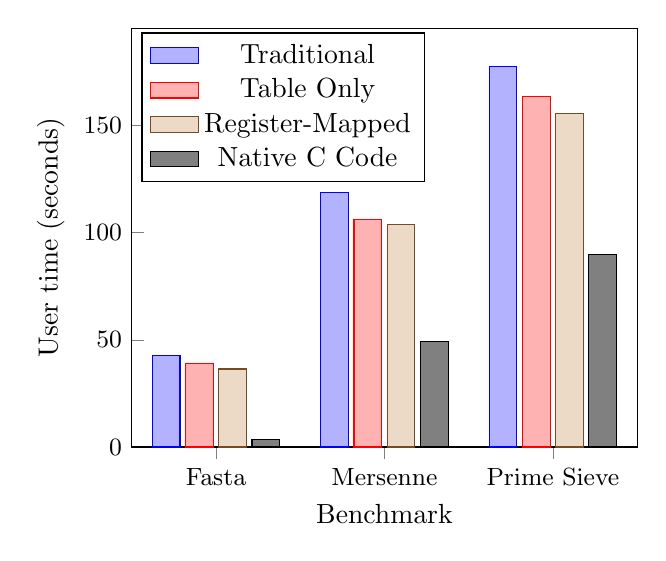
\begin{tikzpicture}
	\begin{axis}[
		ybar,
		xlabel=Benchmark,
		enlarge x limits=0.25,
		ylabel=User time (seconds),
		tickpos=left,
		xticklabels={Fasta,Mersenne,Prime Sieve},
		xtick={2,3,4},
		legend image code/.code={%
			\draw[#1] (0cm,-0.1cm) rectangle (0.6cm,0.1cm);
			},
		legend style={
			at={(0.3,0.99,0)},
			anchor=north,
			legend columns=1},
		tick label style={font=\small},
		ymin=0
		]
	\addplot +[]coordinates {(2,42.771) (3,118.914) (4,177.688)};
	\addplot coordinates {(2,39.148) (3,106.359) (4,163.794)};
	\addplot coordinates {(2,36.4) (3,103.698) (4,155.672)};
	\addplot coordinates {(2,3.373) (3,49.284) (4,89.771)};
	\legend{Traditional,Table Only,Register-Mapped,Native C Code}
	\end{axis}
	\end{tikzpicture}
\end{document}